\subsection{Multiplicadores de Lagrange}

Maximizar $f(x,y)$ quando $(x,y)$ satisfazem a condição $g(x,y)=0$:
\[
\begin{cases}
\text{Maximizar } f(x,y)\\
\text{s.a. } g(x,y)=0
\end{cases}
\]

\begin{figure}[htbp]
  \centering
  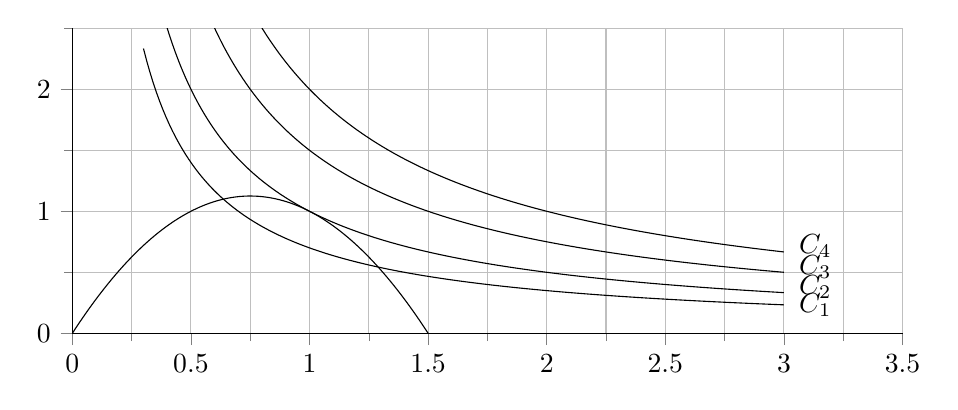
\begin{tikzpicture}
    \begin{axis}[
      width=\linewidth,
      height=0.45\textwidth,
      xmin=0, xmax=3.5,
      ymin=0, ymax=2.5,
      axis x line=bottom,
      axis y line=left,
      axis line style={-},
      tick align=outside,
      grid=both,
      minor tick num=1
    ]
      % C1: 0.7/x
      \addplot[
        domain=0.3:3,
        samples=200
      ] {0.7/x}
        coordinate[pos=1] (Cone);
      \node[anchor=west, xshift=2pt] at (Cone) {$C_1$};

      % C2: 1/x
      \addplot[
        domain=0.3:3,
        samples=200
      ] {1/x}
        coordinate[pos=1] (Ctwo);
      \node[anchor=west, xshift=2pt, yshift=2pt] at (Ctwo) {$C_2$};

      % C3: 1.5/x
      \addplot[
        domain=0.3:3,
        samples=200
      ] {1.5/x}
        coordinate[pos=1] (Cthree);
      \node[anchor=west, xshift=2pt, yshift=2pt] at (Cthree) {$C_3$};

      % C4: 2/x
      \addplot[
        domain=0.3:3,
        samples=200
      ] {2/x}
        coordinate[pos=1] (Cfour);
      \node[anchor=west, xshift=2pt, yshift=2pt] at (Cfour) {$C_4$};

      % curva tangente (exemplo)
      \addplot[domain=0:3, samples=200] {-2*x^2 + 3*x};

    \end{axis}
  \end{tikzpicture}
  \caption{Curvas de nível e tangência (exemplo ilustrativo).}
\end{figure}

\[
\nabla g(P) \perp \text{curva } g=0,
\qquad
\nabla f(P) \perp \text{curva } f=C.
\]

No ponto $P$ que fornece $f_{\max}$ (ou $f_{\min}$) sob a condição $g=0$, as curvas
de nível de $g$ e de $f$ são tangentes. Logo, $\nabla f(P)$ e $\nabla g(P)$ têm a mesma direção,
isto é, são múltiplos.

Assim, existe um número real $\lambda$ tal que
\[
\nabla f(P) = \lambda \, \nabla g(P),
\]
onde $\lambda$ é chamado de \textit{multiplicador de Lagrange}.

Para encontrar máximos e mínimos de $f(x,y)$ sob a restrição $g(x,y)=0$, devemos resolver:
\[
\begin{cases}
\nabla f(x,y) = \lambda \, \nabla g(x,y)\\
g(x,y) = 0
\end{cases}
\]
Isto é:
\[
\begin{cases}
\dfrac{\partial f}{\partial x}(x,y) = \lambda \, \dfrac{\partial g}{\partial x}(x,y) \\[6pt]
\dfrac{\partial f}{\partial y}(x,y) = \lambda \, \dfrac{\partial g}{\partial y}(x,y) \\[6pt]
g(x,y) = 0
\end{cases}
\]

\textbf{Exercício 1.} Determinar, dentre todos os retângulos de 
perímetro $12$, aquele que possui a maior área.

\begin{figure}[htbp]
  \centering
  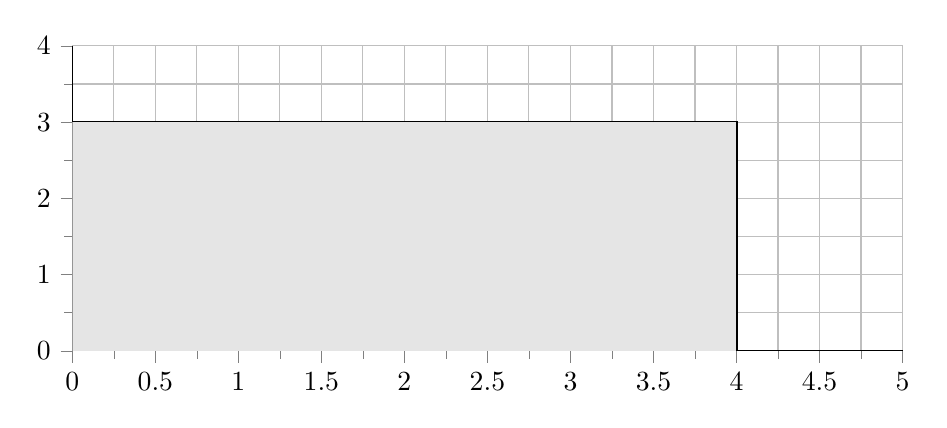
\begin{tikzpicture}
    \begin{axis}[
      width=\linewidth,
      height=0.45\textwidth,
      xmin=0, xmax=5,
      ymin=0, ymax=4,
      axis x line=bottom,
      axis y line=left,
      axis line style={-},
      tick align=outside,
      grid=both,
      minor tick num=1
    ]
      % retângulo exemplo
      \addplot[thick, solid] coordinates {(0,0) (4,0) (4,3) (0,3) (0,0)};
      \addplot[fill=black!10, draw=none]
        coordinates {(0,0) (4,0) (4,3) (0,3)};
    \end{axis}
  \end{tikzpicture}
  \caption{Retângulo com lados $x$ e $y$ (ilustrativo).}
\end{figure}


\[
\begin{cases}
\text{Maximizar } f(x,y) = xy \\
\text{s.a. } g(x,y) = 2x + 2y - 12 = 0
\end{cases}
\]
\textbf{Nota.} $g(x,y)=0$ representa o perímetro fixado em $12$.

Como $\nabla f = (y,x)$ e $\nabla g = (2,2)$, a condição $\nabla f = \lambda \nabla g$ resulta em:
\[
\begin{cases}
y = 2\lambda \\
x = 2\lambda \\
2x + 2y - 12 = 0
\end{cases}
\Rightarrow x = y.
\]
Substituindo na restrição: $2x + 2x = 12 \Rightarrow 4x = 12 \Rightarrow x = 3$, logo $y = 3$.
O retângulo de área máxima é um quadrado de lado $3$, resultando em $x=3$ e $y=3$.

\textbf{Exercício 2.} Calcule os valores máximo ($\operatorname{Max}$) e mínimo ($\operatorname{Min}$) de
$f(x,y) = x^2 - xy + y^2$ sob a restrição $g(x,y) = x^2 + y^2 - 1 = 0$.

Calculando os gradientes:
\[
\nabla f(x,y) = (2x-y, \, -x+2y),
\qquad
\nabla g(x,y) = (2x, \, 2y).
\]
O sistema $\nabla f = \lambda \nabla g$ fornece:
\[
\begin{cases}
2x - y = 2\lambda x \\
-x + 2y = 2\lambda y \\
x^2 + y^2 = 1
\end{cases}
\]

Da primeira equação: $2x - y = 2\lambda x \Rightarrow -y = 2x(\lambda-1) \Rightarrow \boxed{y = 2x(1-\lambda)}$.
Da segunda equação: $-x + 2y = 2\lambda y \Rightarrow -x = 2y(\lambda-1) \Rightarrow \boxed{x = 2y(1-\lambda)}$.

Dividindo as equações (assumindo $xy \neq 0$):
\[
\frac{y}{x} = 2(1-\lambda) \quad \text{e} \quad \frac{x}{y} = 2(1-\lambda) \Rightarrow \frac{y}{x} = \frac{x}{y} \Rightarrow x^2 = y^2.
\]
Com $x^2 + y^2 = 1$, segue que:
\[
x^2 = y^2 = \frac{1}{2} \Rightarrow x = \pm\frac{\sqrt{2}}{2}, \quad y = \pm\frac{\sqrt{2}}{2}.
\]
Os pontos candidatos são $(\pm\sqrt{2}/2, \pm\sqrt{2}/2)$. Deve-se avaliar $f$ em cada ponto para determinar o máximo e o mínimo.

\medskip
\textbf{Exercício 3.} Achar o máximo ($\operatorname{Max}$) e o mínimo ($\operatorname{Min}$) de
$f(x,y) = 2x + 2y - x^2 - y^2$ sob a restrição $(x-2)^2 + y^2 = 2$.

Derivadas parciais:
\[
\begin{cases}
f_x = 2 - 2x \\
f_y = 2 - 2y
\end{cases}
\qquad
\begin{cases}
g_x = 2(x-2) \\
g_y = 2y
\end{cases}
\]

Sistema de Lagrange:
\[
\begin{cases}
2 - 2x = \lambda \, 2(x-2) \Rightarrow (1-x) = \lambda(x-2) \\
2 - 2y = \lambda \, 2y \Rightarrow 1-y = \lambda y \\
(x-2)^2 + y^2 = 2
\end{cases}
\]

Da segunda equação: $\lambda = \frac{1-y}{y}$ (para $y \neq 0$).
Substituindo na primeira:
\[
(1-x) = \frac{1-y}{y}(x-2) \Rightarrow y(1-x) = (1-y)(x-2).
\]
Expandindo:
\[
y - xy = x - 2 - xy + 2y \Rightarrow y = x - 2 + 2y \Rightarrow y = 2 - x.
\]

Aplicando na restrição:
\[
(x-2)^2 + y^2 = 2 \Rightarrow (x-2)^2 + (2-x)^2 = 2 \Rightarrow 2(x-2)^2 = 2 \Rightarrow (x-2)^2 = 1.
\]
Portanto, $x = 2 \pm 1$, resultando em:
\[
x_1 = 3, \, y_1 = -1 \quad \text{e} \quad x_2 = 1, \, y_2 = 1.
\]

Avaliação da função:
\[
f(1,1) = 2+2-1-1 = 2, \qquad f(3,-1) = 6-2-9-1 = -6.
\]
Logo, $f_{\max} = 2$ em $(1,1)$ e $f_{\min} = -6$ em $(3,-1)$.
\newpage


\begin{figure}[p]
  \centering
  \begin{adjustbox}{max width=\linewidth, max totalheight=0.78\textheight, keepaspectratio, center}
    \begin{tikzpicture}[
      node distance=1.0cm,
      >=Stealth,
      every node/.style={font=\scriptsize},
      block/.style={
        rectangle, draw, rounded corners, align=center,
        minimum width=5.6cm, minimum height=0.70cm
      },
      startstop/.style={
        ellipse, draw, align=center,
        minimum width=2.4cm, minimum height=0.65cm
      }
    ]
      \node[startstop] (start) {Início};

    \node[block, below=of start] (def) {Definir \\[2pt]
      $f(x,y) = 2x + 2y - x^2 - y^2$ \\[2pt]
      $g(x,y) = (x-2)^2 + y^2 - 2 = 0$
    };

    \node[block, below=of def] (grad) {Calcular os gradientes \\[2pt]
      $\nabla f = (2-2x, \; 2-2y)$ \\[2pt]
      $\nabla g = (2(x-2), \; 2y)$
    };

    \node[block, below=of grad] (sist) {Montar o sistema de Lagrange \\[2pt]
      $\nabla f = \lambda \nabla g$ \\[2pt]
      $\Rightarrow
        \begin{cases}
          1 - x = \lambda(x-2)\\
          1 - y = \lambda y\\
          (x-2)^2 + y^2 = 2
        \end{cases}$
    };

    \node[block, below=of sist] (solve) {Resolver o sistema \\[2pt]
      $\Rightarrow y = 2 - x$ e $(x-2)^2 = 1$ \\[2pt]
      Pontos candidatos: $(1,1)$ e $(3,-1)$
    };

    \node[block, below=of solve] (eval) {Avaliar $f$ nos pontos \\[2pt]
      $f(1,1) = 2$, \quad $f(3,-1) = -6$
    };

    \node[block, below=of eval] (class) {Classificar \\[2pt]
      Máximo em $(1,1)$ com $f_{\max}=2$ \\[2pt]
      Mínimo em $(3,-1)$ com $f_{\min}=-6$
    };

    \node[startstop, below=of class] (end) {Fim};

    \draw[->] (start) -- (def);
    \draw[->] (def) -- (grad);
    \draw[->] (grad) -- (sist);
    \draw[->] (sist) -- (solve);
    \draw[->] (solve) -- (eval);
    \draw[->] (eval) -- (class);
    \draw[->] (class) -- (end);

    \end{tikzpicture}
  \end{adjustbox}
  \caption{Fluxograma do método dos multiplicadores de Lagrange.}
\end{figure}


